\section{Nozioni di Base}
\label{sec:base}
In questa prima sezione del lavoro intendiamo fornire alcune nozioni di base fondamentali per una piena comprensione dell'argomento; in seguito proporremo la definizione di \emph{bisimulazione}, e ne dedurremo alcune conseguenze immediate che utilizzeremo ampiamente nel seguito della trattazione; proseguiremo illustrando alcune idee che consentono di legare la \emph{bisimulazione} e la teoria degli insiemi; infine concluderemo la sezione introducendo un altro problema, la determinazione della \emph{relational stable coarsest partition}, che come si vedrà è equivalente al problema della bisimulazione. Questa equivalenza avrà un ruolo fondamentale nella Sezione \ref{sec:algs}.

\subsection{Relazioni Binarie}
Riportiamo la definizione di \emph{relazione binaria} \cite{bin_relations} su uno o due insiemi, che sarà utile per definire formalmente il concetto di \emph{grafo}, fondamentale all'interno di questo elaborato:
\begin{definition}
    Una \emph{relazione binaria} su $A,B$ è un sottoinsieme del prodotto cartesiano $A \times B$.\\
    Una \emph{relazione binaria} su $A$ è un sottoinsieme del prodotto cartesiano $A \times A$.\\
	Se $\mathcal{R}$ mette in relazione $u,v$, cioè $(u,v) \in \mathcal{R}$, si usa la notazione $u \mathcal{R} v$ o $\mathcal{R}(u,v)$.
\end{definition}
\begin{definition}
    L' \emph{insieme immagine} di un elemento $x$ dell'insieme $A$ attraverso la relazione $\mathcal{R}$ è l'insieme $\mathcal{R}(x) = \{y \in B \mid x \mathcal{R} y\}$.
\end{definition}
Alcune relazioni binarie dispongono di una o più delle seguenti caratteristiche:
\begin{definition}
    Sia $\mathcal{R}$ una relazione binaria su $A$. Siano $x,y,z$ qualsiasi appartenenti ad $A$. Allora $\mathcal{R}$ è:
    \begin{itemize}
        \item \emph{Riflessiva} se $x \mathcal{R} x$;
        \item \emph{Simmetrica} se $x \mathcal{R} y \implies y \mathcal{R} x$;
        \item \emph{Transitiva} se $(x \mathcal{R} y \land y \mathcal{R} z) \implies x \mathcal{R} z$.
    \end{itemize}
\end{definition}
\begin{example}
    La relazione ``$\leq$'' su $\mathbb{N}$ è riflessiva e transitiva, ma non simmetrica. La relazione ``$=$'' ($a = b \iff $``$a,b$ sono lo stesso numero'') su $\mathbb{N}$ è simmetrica, riflessiva e transitiva.
\end{example}
\begin{definition}
    Una \emph{relazione di equivalenza} su un insieme $A$ è una relazione binaria riflessiva, simmetrica e transitiva. Si vede facilmente che questo genere di relazione partiziona $A$ in \emph{classi di equivalenza}, ovvero sottoinsiemi disgiunti di $A$ all'interno dei quali tutte le coppie di elementi sono in relazione.
\end{definition}
Data una relazione di equivalenza $\mathcal{R}$ su un insieme $A$, si usa la notazione ``$[a]_{\mathcal{R}}$'' per indicare la classe di equivalenza di $\mathcal{R}$ cui appartiene $\mathcal{R}$. Inoltre si usa la notazione ``$A/\mathcal{R}$'', letta ``\emph{quoziente} di $A$ rispetto a $\mathcal{R}$'', per denotare l'insieme delle classi di equivalenza di $\mathcal{R}$ su $A$.\\
In alcune situazioni risulta conveniente definire la più piccola relazione (cioè quella che mette in relazione il minor numero possibile di coppie) che dispone di una certa proprietà, e che contiene una relazione binaria di partenza. Una relazione costruita in questo modo è una ``\emph{chiusura}'':
\begin{definition}
	Sia $\mathcal{R}$ una relazione binaria su $A$. Le seguenti relazioni sono chiusure di $\mathcal{R}$:
    \begin{itemize}
        \item \emph{Riflessiva}: $\mathcal{R}_r = \mathcal{R} \cup \{(x,x) \mid x \in A\}$;
        \item \emph{Simmetrica}: $\mathcal{R}_s = \mathcal{R} \cup \{(y,x) \mid x \mathcal{R} y\}$;
        \item \emph{Transitiva}: $\mathcal{R}_t = \mathcal{R} \cup \{(x,z) \mid \exists y \in A,\, x \mathcal{R} y \land y \mathcal{R} z\}$.
    \end{itemize}
\end{definition}
\begin{example}
    La chiusura riflessiva della relazione ``$<$'' (minore stretto) è la relazione ``$\leq$''.
\end{example}
Nel seguito useremo ampiamente la definizione seguente:
\begin{definition}
    Sia $\mathcal{R}$ una relazione binaria su $A \times B$. La \emph{contro-immagine} di un elemento $y \in B$ rispetto ad $\mathcal{R}$ è l'insieme $\mathcal{R}^{-1}(y) = \{x \in A \mid x \mathcal{R} y\}$.\\
    Più in generale, la \emph{funzione inversa} di $R$ è la funzione $\mathcal{R}^{-1} : \mathcal{P}(B) \to \mathcal{P}(A)$ (dove ``$\mathcal{P}$'' denota l'insieme delle parti) che associa ad un sottoinsieme di $B$ tutti gli $x \in A$ tali che vale $x \mathcal{R} y$ per almeno un $y$ del sottoinsieme.
\end{definition}
Adottiamo infine la notazione ``$|A|$'' per indicare la \emph{cardinalità} dell'insieme $A$. In modo analogo, data una relazione binaria $\mathcal{R}$, $|\mathcal{R}|$ è il numero delle coppie messe in relazione da $\mathcal{R}$.

\subsection{Grafi}
Il problema che intendiamo affrontare in questo elaborato è descritto con il formalismo della teoria dei grafi. In questa sezione presentiamo un sottoinsieme minimale di definizioni e risultati che ci consentirà di introdurre e trattare la questione.

\subsubsection{Definizione e generalità}
Con le premesse viste sopra possiamo definire un \emph{grafo} come segue:
\begin{definition}
    Sia $V$ un insieme finito non vuoto. Sia $E$ una relazione binaria su $V$. La coppia $G = (V, E)$ è un \emph{grafo diretto} (o \emph{orientato}). Con questa notazione:
    \begin{itemize}
        \item $V$ è l'insieme dei \emph{nodi} (o \emph{vertici});
        \item $E$ è una relazione binaria (in generale non simmetrica) che mette in relazione alcuni dei nodi di $G$.
    \end{itemize}
\end{definition}
\begin{example}
    \begin{figure}[t]
        \centering
        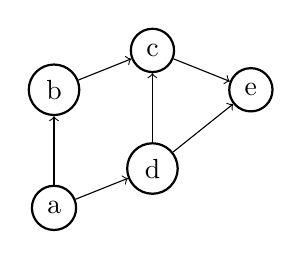
\begin{tikzpicture}[scale=0.5]
            \begin{scope}[every node/.style={circle,thick,draw}]
                \node (a) at (0,0) {a};
                \node (b) at (0,3) {b};
                \node (c) at (2.5,4) {c};
                \node (d) at (2.5,1) {d};
                \node (e) at (5,3) {e};
            \end{scope}

            \begin{scope}
                \path [->] (a) edge node {} (b);
                \path [->] (b) edge node {} (c);
                \path [->] (a) edge node {} (d);
                \path [->] (d) edge node {} (c);
                \path [->] (d) edge node {} (e);
                \path [->] (c) edge node {} (e);
            \end{scope}
            \end{tikzpicture}
        \caption{Rappresentazione grafica di un grafo diretto}
        \label{fig:graph}
    \end{figure}
    Il grafo di Figura \ref{fig:graph} è descritto dalla coppia
    \begin{itemize}
        \item $V = \{a,b,c,d,e\}$
        \item $E = \{(a,b), (a,d), (b,c), (d,c), (c,e), (d,e)\}$
    \end{itemize}
\end{example}
Nel seguito utilizzeremo ampiamente la seguente terminologia:
\begin{definition}
    Sia $G = (V,E)$ un grafo diretto. Consideriamo un arco $(u,v) \in E$. In questo caso $u$ è la \emph{sorgente} dell'arco, mentre $v$ è la \emph{destinazione}. Se il numero di archi uscenti da un nodo è zero, allora tale nodo  è un \emph{pozzo} (dall'inglese \emph{sink}).
\end{definition}

\subsubsection{Componenti fortemente connesse}
Come abbiamo visto sopra, un grafo diretto è un insieme di elementi (i \emph{nodi}) accoppiato con un insieme di relazioni tra questi elementi (gli \emph{archi}). \accente naturale associare questo concetto all'idea di percorso: ogni grafo è definito da un insieme di nodi ed un insieme di \emph{cammini} che consentono di spostarsi da un nodo ad un altro. La seguente definizione sorge in modo spontaneo da questa interpretazione:
\begin{definition}
    Sia $G = (V, E)$ un grafo diretto. Siano $u,v \in V$. $v$ \emph{è raggiungibile} da $u$, o in alternativa \emph{esiste un cammino} da $u$ a $v$, o ancora $u E^{*} v$, se esiste una sequenza finita di nodi $\displaystyle \{x_n\}_{n \in \{0,\dots,K\}}$, tale che $x_0 = u, x_K = v, x_n E x_{n+1}$.
\end{definition}
L'esistenza di un cammino tra nodi fornisce un criterio immediato per partizionare un grafo in gruppi di nodi. Diamo innanzitutto la seguente definizione:
\begin{definition}
    Un grafo diretto $(V,E)$ è \emph{fortemente connesso} se per ogni coppia di nodi $v_1, v_2 \in V$ esiste un cammino da $v_1$ a $v_2$, cioè $v_1 E^{*} v_2$.
\end{definition}
Allora possiamo individuare i sottografi massimali (cioè la ripartizione del grafo in sottografi che consente di minimizzare il numero di sottografi) fortemente connessi (\hspace*{-0.1cm}\cite[Appendice B]{clrs}):
\begin{definition}
    Le \emph{componenti fortemente connesse} (\emph{strongly connected components}, \emph{SCC}) di un grafo diretto sono i sottografi che compongono la ripartizione (massimale) del grafo in sottografi fortemente connessi.
\end{definition}
\begin{example}
    \begin{figure}[t]
        \centering
        \begin{tikzpicture}[scale=0.5]
            \begin{scope}[every node/.style={circle,thick,draw}]
                \node (a) at (0,0) {a};
                \node (b) at (0,3) {b};
                \node (c) at (2.5,4) {c};
                \node (d) at (2.5,1) {d};
                \node (e)[diamond] at (5,3) {e};
            \end{scope}

            \begin{scope}
                \path [->] (a) edge node {} (b);
                \path [->] (b) edge node {} (c);
                \path [->] (d) edge node {} (a);
                \path [->] (c) edge node {} (d);
                \path [->] (d) edge node {} (e);
                \path [->] (c) edge node {} (e);
            \end{scope}
            \end{tikzpicture}
        \caption{SCC di un grafo diretto}
        \label{fig:graph_cfc_1}
    \end{figure}
    Nel grafo di Figura \ref{fig:graph_cfc_1} le SCC sono rappresentate con forme diverse: $\{a,b,c,d\}, \{e\}$.
\end{example}
Il partizionamento dei nodi in SCC è definito come segue:
\begin{definition} \label{def:scc_partition}
    Sia $G = (V, E)$ un grafo diretto. Il grafo $G^{\superscc} = (V^{\superscc}, E^{\superscc})$, dove:
    \begin{itemize}
        \item $V^{\superscc} = \{C \mid \,C$ è una SCC$\}$;
        \item $E^{\superscc} = \{(A,B) \in V^{\superscc} \times V^{\superscc} \mid A \neq B, \exists m \in A, n \in B, m E n\}$
    \end{itemize}
    è il partizionamento del grafo iniziale in SCC.
\end{definition}
Riportiamo la seguente proprietà immediata:
\begin{proposition}
    Sia $G^{\superscc}$ il grafo delle SCC di un grafo $G$ generico. Allora $G^{\superscc}$ è aciclico.
\end{proposition}
\begin{proof2}
    Supponiamo per assurdo che in $G^{\superscc}$ esista un ciclo. Allora tutti i nodi di $V^{\superscc}$ facenti parte del ciclo sono mutuamente raggiungibili (percorrendo il ciclo). Quindi tutti i nodi fanno parte della stessa SCC, ma questo è assurdo.
\end{proof2}
\begin{example}
    \begin{figure}[t]
        \centering
        \begin{subfigure}{.45\textwidth}
          \centering
          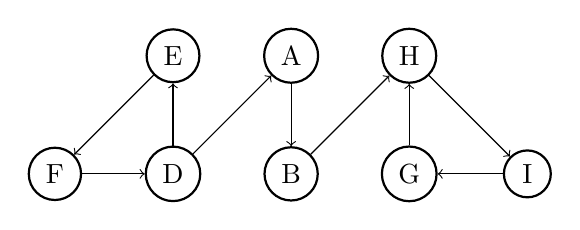
\begin{tikzpicture}[scale=0.5]
            \begin{scope}[every node/.style={circle,thick,draw}]
                \node (A) at (0,3) {A};
                \node (B) at (0,0) {B};

                \node (D) at (-3,0) {D};
                \node (E) at (-3,3) {E};
                \node (F) at (-6,0) {F};

                \node (G) at (3,0) {G};
                \node (H) at (3,3) {H};
                \node (I) at (6,0) {I};
            \end{scope}

            \begin{scope}
                \path [->] (A) edge node {} (B);

                \path [->] (E) edge node {} (F);
                \path [->] (F) edge node {} (D);
                \path [->] (D) edge node {} (E);

                \path [->] (G) edge node {} (H);
                \path [->] (H) edge node {} (I);
                \path [->] (I) edge node {} (G);

                \path [->] (D) edge node {} (A);
                \path [->] (B) edge node {} (H);
            \end{scope}
            \end{tikzpicture}
          \caption{Un grafo}
        \end{subfigure}
        \hfill
        \begin{subfigure}{.45\textwidth}
          \centering
          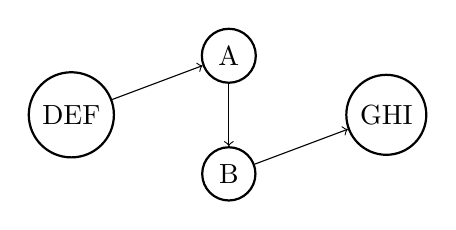
\begin{tikzpicture}[scale=0.5]
            \begin{scope}[every node/.style={circle,thick,draw}]
                \node (A) at (0,3) {A};
                \node (B) at (0,0) {B};

                \node (DEF) at (-4,1.5) {DEF};

                \node (GHI) at (4,1.5) {GHI};
            \end{scope}
                \path [->] (A) edge node {} (B);
                \path [->] (DEF) edge node {} (A);
                \path [->] (B) edge node {} (GHI);
            \begin{scope}

            \end{scope}
            \end{tikzpicture}
          \caption{Corrispondente grafo delle SCC}
        \end{subfigure}
        \caption{Un grafo ed il corrispondente grafo delle SCC}
        \label{fig:graph_cfc_2}
    \end{figure}
    La Figura \ref{fig:graph_cfc_2}.a rappresenta un grafo diretto generico, la Figura \ref{fig:graph_cfc_2}.b rappresenta il suo grafo delle componenti fortemente connesse associato.
\end{example}
Dato un grafo diretto generico possiamo determinare la ripartizione in SCC dei suoi nodi sfruttando un algoritmo avente complessità lineare $\Theta(|V| + |E|)$ \cite{tarjan}. L'algoritmo non verrà trattato in questo elaborato.\\

\subsubsection{Visita in profondità}
Delle due metodologie prevalenti per l'esplorazione di un grafo, \emph{visita in ampiezza} (\emph{Breadth-First-Search}, abbreviato in BFS) e \emph{visita in profondità} (\emph{Depth-First-Search}, abbreviato in DFS), in questo lavoro ci interessiamo alla seconda. Come dice il nome, questa tecnica consiste nella visita esaustiva di tutti i figli di un nodo, prima di passare agli altri nodi sullo stesso livello. Riportiamo lo pseudocodice da \cite{clrs}, leggermente modificato:\\
\begin{algorithm}[H]
    \label{alg:dfs}
    \KwData{$G = (V,E)$}
    \caption{DFS}
    \SetAlgoLined
    \SetKwProg{Fn}{function}{:}{end}
    \Fn{\textup{dsf-visit}($G = (V,E), n,$ time)}{
        n.color = GRAY\;
        \ForAll{$m \mid (nEm \land m.$color = WHITE)}{
            time = dfs-visit($G, m,$ time)\;
        }
        n.finishing-time = time\;
        n.color = BLACK\;
        time = time+1\;
        \Return{time}\;
    }
    \Begin{
        \ForAll{$n \in V$}{
            n.color = WHITE\;
        }

        time = 0\;
        \While{$\exists n \in V \mid n.color ==$ WHITE}{
            time = dfs-visit($G,n,$ time)\;
        }
    }
\end{algorithm}
L'attributo \emph{color} dei nodi del grafo consente di distinguere tra quei nodi che sono già stati visitati in modo esauriente (colore nero), quelli per cui è in corso una visita in profondità (colore grigio) e quelli non ancora esaminati dall'algoritmo (colore bianco). Si osservi che la colorazione dei nodi non è solamente accessoria, ma fornisce un meccanismo per evitare un loop infinito nel caso in cui il grafo contenga un ciclo.

Oltre alla colorazione dei nodi, l'algoritmo imposta l'attributo \emph{finishing-time} per ogni nodo, ovvero l'istante di tempo (a partire da \emph{time} $= 0$) in cui è stata terminata la visita esaustiva in profondità per tale nodo. Nello pseudocodice completo vengono considerati altri due attributi: \emph{starting-time} e \emph{parent}. Questi ultimi tre attributi forniscono alcune importanti proprietà all'algoritmo di visita in profondità, che non saranno approfondite in questo lavoro (si vedano \emph{Parenthesis theorem}, \emph{White-path theorem} in \cite{clrs}).

L'attributo \emph{finishing-time} è sufficiente per alcune applicazioni che saranno esposte nelle sezioni seguenti.

\subsection{Insiemi}
\subsubsection{Cenni di teoria degli insiemi}
In generale supporremo validi gli assiomi su cui si fonda la teoria degli insiemi ZFC, ad eccezione dell'Assioma di Fondazione. Diamo innanzitutto una formulazione degli assiomi che interverranno nel seguito del lavoro:
\begin{axiom}[di estensionalità]
    Due insiemi sono uguali se e solo se contengono gli stessi elementi.
\end{axiom}

\begin{axiom}[di fondazione]
    Ogni insieme non vuoto contiene un elemento disgiunto dall'insieme stesso.
    \label{axi:foundation}
\end{axiom}
Del primo faremo un uso esplicito nel seguito. Il secondo, per motivi che saranno evidenti nella sezione seguente, risulta limitante nell'ambito che intendiamo trattare.

Vale la seguente definizione:
\begin{definition}
    Un insieme è \emph{ben-fondato} se non contiene se stesso. Altrimenti è \emph{non-ben-fondato}.
\end{definition}

\begin{example}
    L'insieme $\Omega = \{\Omega\}$ è non-ben-fondato. L'insieme $A = \{1,2,3\}$ è ben-fondato.
\end{example}

Riportiamo una formulazione equivalente dell'Assioma \ref{axi:foundation} \cite[Chapter III.4]{kunen}:
\begin{axiom*}[\ref*{axi:foundation} bis]
    $\forall A$ la relazione ``$\in$'' è ben-fondata su $A$.
\end{axiom*}

Da questa formulazione risulta evidente l'impossibilità, nel sistema di assiomi ZFC, di costruire insiemi non-ben-fondati.

Rinunciando all'Assioma \ref{axi:foundation} si ottiene un sistema di assiomi che ammette l'esistenza di insiemi non-ben-fondati; tuttavia si può verificare che questo sistema non è più sufficiente a descrivere in modo esaustivo l'aritmetica per mezzo di operazioni su insiemi \cite{aczel}.

Per ovviare a questa mancanza si introduce l'Assioma AFA, che verrà presentato e discusso nella sezione seguente.

% TODO: definisci insieme ereditariamente finito (si può costruire a partire dall'insieme vuoto utilizzando solamente il costruttore {} vedi ZFC) e insime non-ben-fondato prima di usare i grafi per rappresentare gli insiemi

\subsubsection{Rappresentazione di insiemi tramite grafi diretti}
\label{sec:graphs_sets}
In alcuni casi risulta conveniente fornire un'in\-ter\-pre\-ta\-zio\-ne insiemistica della nozione di grafo vista sopra. Introduciamo innanzitutto un concetto fondamentale per il seguito del lavoro:
\begin{definition}
    Sia $G = (V, E)$ un grafo diretto. Supponiamo che esista un $u \in V$ tale che ogni vertice del grafo è raggiungibile da $u$. Allora la coppia $(G, u)$ è un \emph{accessible pointed graph}, o \emph{APG}.
\end{definition}

Per rappresentare un insieme tramite un grafo diretto è necessario passare per un procedimento denominato \emph{decorazione}:
\begin{definition}
    La \emph{decorazione} di un APG è l'assegnazione di un insieme ad ogni suo nodo. In tal caso viene associata la relazione ``$\in$'' alla relazione $E$, ovvero $\langle a,b \rangle \iff b \in a$.
\end{definition}

Possiamo dare la seguente definizione:
\begin{definition}
    L'\emph{immagine} (o \emph{picture}) di un insieme $A$ è la coppia composta da un APG $(G,v)$ e da una sua decorazione in cui a $v$ è associato lo stesso $A$ \cite{aczel}.
\end{definition}

Vale la seguente proposizione \cite{aczel}:
\begin{proposition}
    Ad un APG aciclico è possibile associare un'unica decorazione.
\end{proposition}

Questo risultato non è stato dimostrato nel caso di un APG contenente almeno un ciclo. Per questo motivo viene introdotto il seguente assioma:
\begin{axiom}[AFA, Anti-Foundation-Axiom]
    Ogni APG possiede un'unica decorazione.
\end{axiom}

L'assioma AFA ha un'ovvia conseguenza:
\begin{corollary}
    Ogni APG è immagine di un unico insieme.
\end{corollary}

\begin{example}
    \begin{figure}[t]
        \centering
        \begin{subfigure}{.25\textwidth}
          \centering
          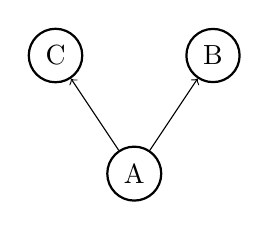
\begin{tikzpicture}[scale=0.5]
            \begin{scope}[every node/.style={circle,thick,draw}]
                \node (A) at (0,0) {A};
                \node (B) at (2,3) {B};
                \node (C) at (-2,3) {C};
            \end{scope}

            \begin{scope}
                \path [->] (A) edge node {} (B);
                \path [->] (A) edge node {} (C);
            \end{scope}
            \end{tikzpicture}
          \caption{$B = \{\emptyset\}$}
          \label{fig:sets_graphs_a}
        \end{subfigure}
        \begin{subfigure}{.15\textwidth}
            \centering
            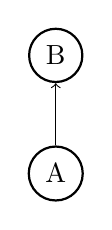
\begin{tikzpicture}[scale=0.5]
              \begin{scope}[every node/.style={circle,thick,draw}]
                  \node (A) at (0,0) {A};
                  \node (B) at (0,3) {B};
              \end{scope}

              \begin{scope}
                  \path [->] (A) edge node {} (B);
              \end{scope}
              \end{tikzpicture}
            \caption{$B = \{\emptyset\}$}
            \label{fig:sets_graphs_b}
          \end{subfigure}
        \begin{subfigure}{.15\textwidth}
          \centering
          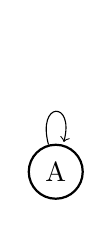
\begin{tikzpicture}[scale=0.5]
            \begin{scope}[every node/.style={circle,thick,draw}]
                \node (A) at (0,-0.3) {A};
                \node[draw=white] (B) at (0,3) {};
            \end{scope}

            \begin{scope}
                \path [->] (A) edge [loop above] node {} (A);
            \end{scope}
            \end{tikzpicture}
          \caption{$A = \{A\}$}
          \label{fig:sets_graphs_c}
        \end{subfigure}
        \begin{subfigure}{.25\textwidth}
            \centering
            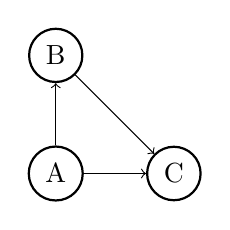
\begin{tikzpicture}[scale=0.5]
              \begin{scope}[every node/.style={circle,thick,draw}]
                  \node (A) at (0,0) {A};
                  \node (B) at (0,3) {B};
                  \node (C) at (3,0) {C};
              \end{scope}

              \begin{scope}
                  \path [->] (A) edge node {} (B);
                  \path [->] (B) edge node {} (C);
                  \path [->] (A) edge node {} (C);
              \end{scope}
              \end{tikzpicture}
            \caption{$A = \{\emptyset, \{\emptyset\}\}$}
            \label{fig:sets_graphs_d}
          \end{subfigure}

        \caption{Rappresentazione di insiemi tramite grafi.}
        \label{fig:graph_set}
    \end{figure}
    In Figura \ref{fig:graph_set} sono rappresentati alcuni insiemi sotto forma di APG. Nella Figura \ref{fig:sets_graphs_a} $B,C$ non hanno nodi figli, sicchè rappresentano l'insieme vuoto, e dunque $A$ è l'insieme che contiene solamente l'insieme vuoto; analogamente si interpreta la Figura \ref{fig:sets_graphs_b}; nella Figura \ref{fig:sets_graphs_c} abbiamo un nodo $A$ il cui unico figlio è lo stesso $A$, sicchè contiene solamente se stesso; infine nella Figura \ref{fig:sets_graphs_d} abbiamo un nodo $C$ che rappresenta l'insieme vuoto, un nodo $B$ che contiene solamente l'insieme vuoto, ed un nodo $A$ che contiene l'insieme vuoto è l'insieme rappresentato da $B$. Associazioni del tipo ``$B$ rappresenta l'insieme vuoto'' sono \emph{decorazioni}.
\end{example}

\subsection{Bisimulazione}
In questa sezione introdurremo la definizione di \emph{bisimulazione} ed alcune proprietà. Proseguiremo con la definizione di \emph{massima bisimulazione}, ed infine proporremo alcune osservazioni che legano la bisimulazione e la teoria degli insiemi.

\subsubsection{Definizione e risultati preliminari}
\begin{definition}
    Siano $G_1 = (V_1,E_1), G_2 = (V_2,E_2)$ due grafi diretti. Una relazione binaria $\mathcal{R}: V_1 \times V_2$ è una \emph{bisimulazione} su $G_1, G_2$ se $\forall a \in V_1, b \in V_2$ valgono congiuntamente le seguenti proprietà:
    \begin{itemize}
        \item $a \mathcal{R} b, \langle a, a' \rangle_{E_1} \implies \exists b' \in V_2 \mid a' \mathcal{R} b' \land \langle b, b' \rangle_{E_2}$
        \item $a \mathcal{R} b, \langle b, b' \rangle_{E_2} \implies \exists a' \in V_1 \mid a' \mathcal{R} b' \land \langle a, a' \rangle_{E_1}$
    \end{itemize}
    Analogamente si definisce una bisimulazione su un unico grafo diretto $G$, ponendo $G_1 = G_2 = G$.
\end{definition}

Nei prossimi paragrafi osserveremo che l'esistenza di una bisimulazione tra due grafi è un'informazione rilevante se siamo interessati agli insiemi che rappresentano.
\begin{definition}
    Siano $G_1 = (V_1,E_1), G_2 = (V_2,E_2)$ due grafi. Essi sono \emph{bisimili} se esiste una bisimulazione su $G_1, G_2$.
    Due APG $(G_1, v_1), (G_2, v_2)$ sono \emph{bisimili} se $G_1, G_2$ sono bisimili e vale $v_1 \mathcal{R} v_2$ per almeno una bisimulazione $\mathcal{R}$ su $G_1, G_2$.
\end{definition}

\begin{observation}
    Una bisimulazione può non essere riflessiva, simmetrica, nè transitiva.
\end{observation}

\begin{example}
    La relazione $a R b \iff$ ``$a,b$ sono lo stesso nodo'' su un grafo qualsiasi è una bisimulazione riflessiva, simmetrica e transitiva.

    La relazione $R = \emptyset$ è una bisimulazione su un grafo qualsiasi, ma non è riflessiva.

    La relazione $R = \{(a,a),(b,b),(c,c),(d,d),(a,b),(b,c),(c,d)\}$ sul grafo $G = (\{a,b,c,d\}, \{(a,b),(b,c),(c,d),(d,d)\})$ è una bisimulazione, ed è solamente riflessiva.
\end{example}

Dalla definizione di bisimulazione possiamo dedurre una proprietà interessante delle chiusure:
\begin{theorem}
    Sia $\mathcal{R}$ una bisimulazione sul grafo diretto $G$. La sua chiusura riflessiva, simmetrica o transitiva è ancora una bisimulazione su $G$.
    \label{theo:bisi_chiusura}
\end{theorem}
\begin{proof2}
    Consideriamo separatamente le tre relazioni $\mathcal{R}_r, \mathcal{R}_s, \mathcal{R}_t$, rispettivamente la chiusura riflessiva, simmetrica e transitiva. Per ogni caso consideriamo solamente le coppie aggiunte dalla chiusura:
    \begin{itemize}
        \item $\mathcal{R}_r$: Per definizione $\mathcal{R} \subseteq \mathcal{R}_r$, quindi è sufficiente dimostrare che $\mathcal{R}_r$ è una bisimulazione quando gli argomenti $u,v \in V$ non sono distinti.

        Sia $u \in V$. Chiaramente per definizione di $\mathcal{R}_r$ si ha $u \mathcal{R}_r u$. Ma $\forall u' \in V \mid \langle u, u' \rangle$ vale (sempre per definizione di $\mathcal{R}_r$) $u' \mathcal{R}_r u'$.
        \item $\mathcal{R}_s$: Per definizione $\mathcal{R} \subset \mathcal{R}_s$, quindi è sufficiente dimostrare che $\mathcal{R}_s$ è una bisimulazione quando per $u,v \in V$ si ha $u \mathcal{R} v$ ma non $v \mathcal{R} u$.

        Sia $(u,v) \in V\times V$. Allora:
        \begin{center}
            $u \mathcal{R}_s v \implies u \mathcal{R} v \lor v \mathcal{R} u$
        \end{center}
        Supponiamo ad esempio che $v \mathcal{R} u$.
        \begin{align*}
            &\implies \forall v' \in V \mid \langle v, v' \rangle \,\,\exists u' \in V, \langle u, u' \rangle \land v' \mathcal{R} u'\\
            &\implies u' \mathcal{R}_s v'
        \end{align*}
        e
        \begin{align*}
            &\implies \forall u' \in V\mid \langle u, u' \rangle \,\,\exists v' \in V, \langle v, v' \rangle \land v' \mathcal{R} u'\\
            &\implies u' \mathcal{R}_s v'
        \end{align*}
        cioè sono dimostrate le due condizioni caratteristiche della bisimulazione.\\
        La dimostrazione è analoga se $u \mathcal{R} v$.
        \item $\mathcal{R}_t$: Per definizione $b \subset \mathcal{R}_t$, quindi è sufficiente dimostrare che $\mathcal{R}_t$ è una bisimulazione quando per gli argomenti $u,v,z \in V$ si ha $u \mathcal{R} v$, $v \mathcal{R} z$ ma non $u \mathcal{R} z$.\\
        Sia $(u,v,z) \in V^3$ una terna con questa proprietà. Allora:
        \begin{gather*}
            \forall u' \in V\mid \langle u, u' \rangle \,\, \exists v' \in V, \langle v, v' \rangle \land u' \mathcal{R} v'
        \end{gather*}
        Inoltre $\exists z' \mid \langle z, z' \rangle \land v' \mathcal{R} z'$.\\
        Riordinando si ha $u' \mathcal{R} v', v' \mathcal{R} z'$. Allora per definizione di $b_t, \, u' \mathcal{R}_t z'$.\\
        In modo speculare si ottiene la seconda condizione caratteristica della bisimulazione.
    \end{itemize}
    \vspace*{-0.75cm}
\end{proof2}

Da questa proposizione si deduce il seguente corollario, che risulta dall'applicazione iterata delle tre chiusure viste in precedenza:
\begin{corollary}
    Ad ogni bisimulazione $\mathcal{R}$ è possibile associare una bisimulazione $\widetilde{\mathcal{R}} \supseteq \mathcal{R}$ che è anche una relazione di equivalenza (Definizione \emph{\ref{def:eq_rel}}).
    \label{cor:bisimulation_eqrel}
\end{corollary}

Concludiamo la sezione relativa ai risultati generali sulla bisimulazione con la seguente proposizione, che sarà utile nel seguito:
\begin{proposition}
    Siano $\mathcal{R}_1, \mathcal{R}_2$ due bisimulazioni su $G_1, G_2$. Allora $\mathcal{R} = \mathcal{R}_1 \cup \mathcal{R}_2$ è ancora una bisimulazione.
    \label{obs:bisimulation_union}
\end{proposition}
\begin{proof2}
    Siano $u,v \mid u \mathcal{R} v$; allora deve valere $u \mathcal{R}_1 v \lor u \mathcal{R}_2 v$. Sia $u' \mid \langle u, u' \rangle$. Ma quindi $\exists v' \mid \langle v,v' \rangle \land u' \mathcal{R}_{1|2} v'$.
\end{proof2}

\subsubsection{Massima bisimulazione}
\label{sec:bisi_max}
Definiamo ora il concetto di \emph{massima bisimulazione}, che sarà l'argomento principale di questo elaborato:
\begin{definition}
    Una bisimulazione $\mathcal{R}_M$ su $G_1, G_2$ è la \emph{bisimulazione massima} su $G_1, G_2$ se per ogni bisimulazione $\mathcal{R}$ su $G_1,G_2 \,\, u \mathcal{R} v \implies u \mathcal{R}_M v$, o equivalentemente $\mathcal{R}_M \supseteq \mathcal{R}$ per ogni bisimulazione $\mathcal{R}$ su $G_1, G_2$.
\end{definition}

\begin{observation}
    Sia $\mathcal{R}_M$ la massima bisimulazione su un grafo diretto $G$. Allora per ogni bisimulazione $\mathcal{R}$ su $G$ si ha $|\mathcal{R}_M| \geq |\mathcal{R}|$.
\end{observation}

Naturalmente la massima bisimulazione dipende dai due grafi presi in esame. Deduciamo alcune caratteristiche immediate:
\begin{proposition}
    Valgono le seguenti proprietà:
    \begin{enumerate}
        \item La massima bisimulazione su due grafi $G_1,G_2$ è unica;
        \item La massima bisimulazione è una relazione di equivalenza.
    \end{enumerate}
    \vspace*{-0.3cm}
    \label{prop:bisi_max_equi}
\end{proposition}
\begin{proof2}
    Le proprietà seguono dal Corollario \ref{cor:bisimulation_eqrel} e dall'Osservazione \ref{obs:bisimulation_union}:
    \begin{enumerate}
        \item Supponiamo per assurdo che esistano due massime bisimulazioni $\mathcal{R}_{M_1}, \mathcal{R}_{M_2}$. La loro unione è ancora una bisimulazione per l'Osservazione \ref{obs:bisimulation_union}, ed ha cardinalità maggiore (se così non fosse le due bisimulazioni coinciderebbero).
        \item Se per assurdo la massima bisimulazione non fosse una relazione di equivalenza, potremmo considerare la sua chiusura riflessiva, simmetrica e transitiva, che avrebbe cardinalità maggiore o uguale alla supposta massima bisimulazione e sarebbe per costruzione una relazione di equivalenza.
    \end{enumerate}
    \vspace*{-0.7cm}
\end{proof2}
Naturalmente il concetto di \emph{massima bisimulazione} può essere definito anche su unico grafo diretto $G$. Questo caso si rivelerà di grande interesse nel seguito. Per ora dimostriamo il seguente risultato:
\begin{theorem}
    Sia $G=(V,E)$ un grafo diretto finito. Allora esiste la massima bisimulazione su $G$.
\end{theorem}
\begin{proof2}
    Può esistere solamente un numero finito di relazioni binarie su $G$, e questo numero fornisce un limite superiore al numero massimo di bisimulazioni su $G$.
    Allora possiamo considerare l'unione di questo numero finito di bisimulazioni, che sarà chiaramente la massima bisimulazione.

    Abbiamo almeno una bisimulazione non banale (ovvero diversa da $\emptyset$) che possiamo ricavare dalla chiusura riflessiva di $\emptyset$ (Teorema \ref{theo:bisi_chiusura}), ovvero la relazione $\mathcal{R} = \{(u,u) \mid u \in V\}$.
\end{proof2}

\subsubsection{Interpretazione insiemistica della bisimulazione}
Mostriamo ora una conseguenza diretta dell'Assioma di Estensionalità e di AFA (Sezione \ref{sec:graphs_sets}):
\begin{theorem}
    Due APG rappresentano lo stesso insieme se e solo se sono bisimili.
    \label{theo:bisi_iff_eqsets}
\end{theorem}
\begin{proof2}
    Siano $G_A = (V_A, E_A), G_B = (V_B, E_B)$. Dimostriamo separatamente le due implicazioni:
    \begin{enumerate}
        \item[$(\implies)$] Osserviamo innanzitutto che la relazione binaria $\equiv \,: V_A \times V_B$ definita come:
        \begin{gather*}
            a \equiv b \iff ``\text{le decorazioni di } G_A,G_B \text{ associano ad } a,b \text{ lo stesso insieme}''
        \end{gather*}
        è una bisimulazione sui grafi $G_A, G_B$.\\
        Chiaramente se $a \equiv b$ e $\langle a, a' \rangle$ si ha:
        \begin{itemize}
            \item $a' \in a$, associando ad $a,a'$ gli insiemi che rappresentano secondo la decorazione (unica per AFA);
            \item $a,b$ rappresentano lo stesso insieme.
        \end{itemize}
        Quindi per l'Assioma di Estensionalità $\exists b' \in b\mid b',a'$ rappresentano lo stesso insieme, cioè $\langle b, b' \rangle$ e $a' \equiv b'$. Si procede specularmente per la seconda condizione caratteristica della bisimulazione.\\
        La relazione ``$\equiv$'' è quindi una bisimulazione sugli APG $G_A,G_B$ quando si assume per ipotesi che rappresentino lo stesso insieme.
        \item[$(\impliedby)$] Sia $\mathcal{R}$ una bisimulazione su $G_A,G_B$. Consideriamo la decorazione $d_A$ (l'unica) di $G_A$. Vogliamo definire una decorazione per $G_B$, e dimostrare che i due grafi con le rispettive decorazioni sono due immagini dello stesso insieme. Dalla possibilità di operare questo procedimento, dall'Assioma di Estensionalità e da AFA potremo dedurre l'uguaglianza degli insiemi rappresentati.

        Definiamo la decorazione $d_B$ come segue:
        \begin{gather*}
            d_B(v) = d_A(u), \text{con $u$ nodo di $G_A$} \mid u \mathcal{R} v
        \end{gather*}
        \begin{observation*}
            Per ogni nodo $v$ di $B$ deve esistere almeno un nodo $u$ di $G_A \mid u \mathcal{R} v$ perchè si suppone che i due APG siano bisimili.
        \end{observation*}
        Dimostriamo che $d_B$ è una decorazione di $G_B$. In altre parole vogliamo dimostrare che per ogni nodo $v$ di $G_B$ l'insieme $d_B(v)$ contiene tutti e soli gli insiemi $d_B(v')$ dove $v'$ è figlio di $v$.
        \begin{itemize}
            \item Supponiamo per assurdo che tra i figli di $v$ ``manchi" il nodo corrispondente ad un elemento $X \in d_B(v)$. Poichè la decorazione di $G_A$ è ben definita, il nodo $u$ di $G_A \mid u \mathcal{R} v$ deve avere un figlio corrispondente a $X$, che chiameremo $u'$, per cui vale quindi $d_A(u') = X$. Ma $u \mathcal{R} b \land \langle u, u' \rangle \implies \exists v' \mid \langle v, v' \rangle, u' \mathcal{R} v'$. Cioè $d_B(v') = d_A(u') = X$. Dunque il nodo mancante è stato trovato.
            \item Supponiamo per assurdo che tra i figli di $v$ ci sia un nodo ``in più'', ovvero un nodo $v' \mid \langle v, v' \rangle$ e $d_B(v') = Y$ con $Y \notin d(v)$. Ma allora, considerando un nodo $u$ di $G_A \mid u \mathcal{R} v$, dovrebbe esistere un $u' \mid \langle u, u' \rangle$ e $u' \mathcal{R} v'$, cioè $d_A(u') = d_B(v') = Y$.
            Ma allora $Y \in d_A(u) = d_B(v)$, deduzione che è chiaramente in contrasto con l'ipotesi.
        \end{itemize}
        \accente possibile che ci siano due nodi di $a_1, a_2$ di $G_A$ ed un nodo $b$ di $G_B$ per cui vale $a_1 \mathcal{R} b \land a_2 \mathcal{R} b$. In questo caso la decorazione definita è ambigua. Per questo motivo correggiamo la formulazione di $d_B$ come segue:
        \begin{gather*}
        d_B(v) = X \text{, dove $X$ è l'insieme associato al nodo $u$ di $A$} \mid u \mathcal{R} v, \\
        \text{con $u$ preso casualmente tra i nodi di $G_A$ bisimili a $v$.}
        \end{gather*}
        Per AFA esiste un'unica decorazione di $G_B$, quindi si deve avere, alternativamente, per ogni nodo $v$ di $G_B$:
        \begin{itemize}
            \item $\exists ! u \in V_A \mid u \mathcal{R} v$;
            \item $\forall u \in V_A \mid u \mathcal{R} v$, la decorazione di $G_A$ associa a tutti gli $u$ lo stesso insieme.
        \end{itemize}
        Dunque l'ambiguità è risolta.
    \end{enumerate}
    \vspace*{-0.75cm}
\end{proof2}
Tenendo conto di quanto affermato nella sezione \ref{sec:graphs_sets}, il Teorema \ref{theo:bisi_iff_eqsets} dimostra che la bisimulazione può sostituire la relazione di uguaglianza tra insiemi quando questi sono rappresentati con APG \cite{dovier}.

Dopo questa considerazone possiamo dare la seguente definizione:
\begin{definition}
    \label{def:bisi_contraction}
    Sia $\mathcal{R}$ una bisimulazione su $G = (V,E)$, dove $G$ è un grafo diretto. Supponiamo che $\mathcal{R}$ sia una relazione di equivalenza. Il grafo, definito a partire dal grafo iniziale, ottenuto con una \emph{contrazione rispetto alla bisimulazione} $\mathcal{R}$ \cite{gentilini}, è il grafo diretto $G_{\mathcal{R}} = (V_{\mathcal{R}}, E_{\mathcal{R}})$:
    \begin{itemize}
        \item $V_{\mathcal{R}} = \{[m]_{\mathcal{R}}, m \in V\}$;
        \item $\langle [m]_{\mathcal{R}}, [n]_{\mathcal{R}} \rangle \in E_{\mathcal{R}} \iff \exists b \in [m]_{\mathcal{R}}, c \in [n]_{\mathcal{R}} \mid \langle b, c \rangle \in E$.
    \end{itemize}
    Si chiama \emph{classe} del nodo $a$ rispetto alla bisimulazione $\mathcal{R}$, indicata con la notazione $[a]_{\mathcal{R}}$, il nodo di $V_{\mathcal{R}}$ in cui viene inserito il nodo $a$.
\end{definition}

La Definizione \ref{def:bisi_contraction} è di fondamentale importanza per la seguente osservazione:
\begin{proposition}
    Sia $G$ un grafo diretto, e sia $G_{\mathcal{R}}$ come nella Definizione \ref{def:bisi_contraction}, per una bisimulazione $R$ qualsiasi. Allora $G, G_{\mathcal{R}}$ sono bisimili.
    \label{prop:bisi_cont_bisi}
\end{proposition}
\begin{proof2}
    Sia ``$\equiv$'' la relazione binaria su $V\times V_{\mathcal{R}}$ definita come segue:
    \begin{gather*}
        m \equiv M \iff M = [m]_{\mathcal{R}}
    \end{gather*}
    Vogliamo dimostrare che tale relazione è una bisimulazione sui grafi $G, G_{\mathcal{R}}$. Supponiamo che $x \equiv X$, e che $\langle x,y \rangle \in E$ per qualche $y \in V$. Chiamiamo $Y \coloneqq [y]_{\mathcal{R}}$. Allora, per la Definizione \ref{def:bisi_contraction}, si ha $\langle X, Y \rangle \in E_{\mathcal{R}}$. Inoltre vale banalmente $y \equiv Y$.

    Per dimostrare la seconda condizione caratteristica della bisimulazione, supponiamo che $x \equiv X$, e che $\langle X, Y \rangle \in E_{\mathcal{R}}$ per qualche $Y \in V_{\mathcal{R}}$. Sempre per la Definizione \ref{def:bisi_contraction} deve esistere un $y \in Y \mid (y \equiv Y \land \langle x, y \rangle \in E)$.
\end{proof2}

La Proposizione \ref{prop:bisi_cont_bisi} ha una conseguenza ovvia, che risulta evidente dal Teorema \ref{theo:bisi_iff_eqsets}:
\begin{corollary}
    Sia $R$ una bisimulazione che sia anche una relazione di equivalenza. Allora l'APG $(G, v)$ e l'APG $(G_R, [v]_R)$ rappresentano lo stesso insieme.
\end{corollary}

Possiamo quindi sfruttare le proprietà della bisimulazione per rappresentare insiemi in una forma minimizzata: è sufficiente ricavare una bisimulazione (che sia anche una relazione di equivalenza) sul grafo che rappresenta l'insieme.

Poichè in generale un grafo ammette più di una bisimulazione (che sia anche una relazione di equivalenza), definiamo una relazione d'ordine sulle rappresentazioni:
\begin{definition}
    La rappresentazione $(G_a, v_a)$ di un insieme è \emph{minore} della rappresentazione equivalente $(G_b, v_b)$ se $|Va| < |Vb|$.

    Una rappresentazione è \emph{minima} se non esiste una rappresentazione equivalente minore.
\end{definition}

\begin{observation}
    La \emph{contrazione per bisimulazione} è una rappresentazione minore (o eventualmente uguale) di quella iniziale.
\end{observation}

Concludiamo la sezione con il seguente risultato, che stabilisce in modo univoco la bisimulazione prescelta per minimizzare la rappresentazione di un dato insieme:
\begin{theorem}
    Sia $(G,v)$ un APG rappresentante un insieme. Sia $\mathcal{R}_M$ la massima bisimulazione su $(G,v)$. Allora la contrazione per bisimulazione indotta da $\mathcal{R}_M$ su $(G,v)$ fornisce la rappresentazione minima dell'insieme.
\end{theorem}
\begin{proof2}
    Supponiamo per assurdo che esista una bisimulazione $\mathcal{R}_V$ su $(G,v)$ che fornisce una contrazione avente un numero di nodi strettamente inferiore alla contrazione indotta da $\mathcal{R}_M$. Ma questo implica che esistono almeno due nodi di $G$ che sono in relazione secondo $\mathcal{R}_V$ e non secondo $\mathcal{R}_M$. Chiaramente questa deduzione è in contrasto con il fatto che $\mathcal{R}_M$ è la massima bisimulazione.

    Supponiamo per assurdo che, dopo la contrazione indotta da $\mathcal{R}_M$, sia possibile trovare una nuova bisimulazione $\mathcal{R}_O$ su $(G_{\mathcal{R}_M}, [v]_{\mathcal{R}_M})$ che induca una contrazione avente un numero di nodi strettamente inferiore a quello di $(G_{\mathcal{R}_M}, [v]_{\mathcal{R}_M})$. Chiaramente $\mathcal{R}_O \subset V_{\mathcal{R}_M} \times V_{\mathcal{R}_M}$.

    Definiamo una nuova bisimulazione $\mathcal{R}_{\widetilde{M}} \subset V\times V$ tale che
    \begin{gather*}
        x \mathcal{R}_{\widetilde{M}} y \iff (x \mathcal{R}_M y \lor [x]_{\mathcal{R}_M} \mathcal{R}_O [y]_{\mathcal{R}_M})
    \end{gather*}
    Per definizione di massima bisimulazione è necessario che valga $\mathcal{R}_{\widetilde{M}} \subset \mathcal{R}_M$, quindi non è possibile che la contrazione indotta da $\mathcal{R}_O$ sia una rappresentazione minore di quella indotta da $\mathcal{R}_M$.
\end{proof2}

\subsection{Relational stable coarsest partition}
\label{sec:rscp}
In questa sezione introdurremo il concetto di \emph{Relational Stable Coarsest Partition} (nel seguito abbreviato in \emph{RSCP}). Nel seguito del lavoro evidenzieremo il legame tra questo problema e quello della determinazione della massima bisimulazione, sfruttato ampiamente dagli algoritmi che tratteremo nel seguito in quanto la formulazione del primo lo rende un problema più facilmente approcciabile dal punto di vista algoritmico.

Cominciamo con alcune definizioni di base:
\begin{definition}
    Sia $S$ un insieme finito. Sia $\mathfrak{X} = \{x_1, \dots, x_n\}$ con $x_i \subseteq S \,\,\,\forall i \in \{1,\dots,n\}$. $\mathfrak{X}$ è una \emph{partizione} di $S$ se:
    \begin{gather*}
        \bigcup_{i = 1}^n x_i = A \qquad \land \qquad x_i \cap x_j = \emptyset \,\,\forall i,j \in \{1,\dots,n\} \qquad \land \qquad x_i \neq \emptyset \,\,\forall i
    \end{gather*}
    Inoltre gli insiemi $x_i$ sono i \emph{blocchi} della partizione $\mathfrak{X}$. Se $a \in x_i$ si usa la notazione $[a]_{\mathfrak{X}} = x_i$.
\end{definition}

\begin{observation}
    \label{obs:part_banale}
    Ogni insieme $S$ ha una partizionamento banale, consistente in un unico blocco contenente tutti gli elementi dell'insieme.
\end{observation}

\begin{example}
    Sia $S \coloneqq \{0,1,2,3,4,5,6\}$. Alcuni possibili partizionamenti sono $\{S\}$ (il partizionamento banale), $\mathfrak{S}_1 = \{\{0,1,2,3\},\{4,5,6\}\}, \mathfrak{S}_2 = \{\{0,1\},\{2,3\},\{4,5,6\}\}$.
    \label{exa:set_partition}
\end{example}

\begin{definition}
    Siano $\mathfrak{X}_1,\mathfrak{X}_2$ due partizioni dello stesso insieme. $\mathfrak{X}_2$ \emph{rifinisce} $\mathfrak{X}_1$ se $\forall x_2 \in \mathfrak{X}_2, \,\,\exists x_1 \in \mathfrak{X}_1 \mid x_2 \subseteq x_1$.
\end{definition}

\begin{example}
    Riprendendo l'Esempio \ref*{exa:set_partition}, la partizione $\mathfrak{S}_2$ rifinisce $\mathfrak{S}_1$, che a sua volta rifinisce la partizione banale.
\end{example}

Il partizionamento di insiemi finiti assume interesse nell'ambito trattato in questo lavoro quando viene introdotta la seguente condizione:
\begin{definition}
    Sia $S$ un insieme, ed $\mathcal{R}$ una relazione binaria su $S$. Sia $\mathfrak{X}$ una partizione di $S$, e sia $B \subseteq S$.
    \begin{itemize}
        \item $\mathfrak{X}$ è \emph{stabile} rispetto alla coppia $(B,\mathcal{R})$ se $\forall x \in \mathfrak{X}$ vale $x \subseteq \mathcal{R}^{-1}(B) \lor x_i \cap \mathcal{R}^{-1}(B) = \emptyset$;
        \item La partizione $\mathfrak{X}$ è \emph{stabile} rispetto ad $\mathcal{R}$ se è stabile rispetto a $(x,\mathcal{R}) \,\,\forall x \in \mathfrak{X}$.
    \end{itemize}
\end{definition}

\begin{example}
    \label{exa:set_partition_stable}
    Consideriamo la relazione binaria $\mathcal{R}$ su $S$ che mette in relazione le coppie $\{(0,1),(1,0),(2,3),(3,2),(4,5),(5,6),(0,4),(1,5)\}$. $\mathfrak{S}_2$ è stabile rispetto a $\mathcal{R}$; $\mathfrak{S}_1$ invece non è stabile rispetto a $\mathcal{R}$.
\end{example}

In altre parole per ogni coppia di blocchi di una partizione stabile si hanno due alternative:
\begin{itemize}
    \item Tutti gli elementi del primo blocco sono in relazione con almeno un elemento del secondo blocco;
    \item Nessuno degli elementi del primo blocco è in relazione con qualche elemento del secondo blocco.
\end{itemize}

Vale il seguente risultato:
\begin{proposition}
    \label{prop:rifi_stabile}
    Sia $\mathfrak{S}$ una partizione qualsiasi di un insieme $S$, e siano $P,Q \subseteq S$. Sia $\mathcal{R}$ una relazione binaria su $S$. Supponiamo $\mathfrak{S}$ stabile rispetto alle coppie $(\mathcal{R},P),(\mathcal{R},Q)$. Allora:
    \begin{enumerate}
        \item Qualsiasi rifinitura di $\mathfrak{S}$ resta stabile rispetto alla coppia $(\mathcal{R},P)$;
        \item $\mathfrak{S}$ è stabile rispetto alla coppia $(\mathcal{R},P \cup Q)$.
    \end{enumerate}
\end{proposition}
\begin{proof2}
    Dimostriamo separatamente i due enunciati:
    \begin{enumerate}
        \item Chiaramente se per un blocco qualsiasi $x \in \mathfrak{S}$ vale $x \subseteq \mathcal{R}^{-1}(P) \lor x \cap \mathcal{R}^{-1}(P) = \emptyset$, la stessa relazione vale per qualsiasi sottoinsieme di $x$;
        \item Sia $x \in \mathfrak{S}$. Chiaramente vale $\mathcal{R}^{-1}(P),\mathcal{R}^{-1}(Q) \subseteq \mathcal{R}^{-1}(P \cup Q)$. Allora, se almeno uno tra $\mathcal{R}^{-1}(P),\mathcal{R}^{-1}(Q)$ contiene l'immagine di $x$ si avrà $x \subseteq \mathcal{R}^{-1}(P \cup Q)$, altrimenti $x \cap \mathcal{R}^{-1}(P \cup Q)$ dovrà chiaramente essere vuoto.
    \end{enumerate}
    \vspace*{-0.75cm}
\end{proof2}

\accente evidente che l'ultimo punto può essere esteso in modo molto semplice all'unione di più sottoinsiemi di $S$. In altre parole, se $\mathfrak{S}$ è stabile rispetto alle coppie $(\mathcal{R},S_i), S_i \subset S, i = 1, \dots, n$, allora è stabile anche rispetto alla coppia $(\mathcal{R}, \bigcup_{i=1}^{n} S_i)$.

Con queste premesse possiamo definire il problema della determinazione della \emph{RSCP}:
\begin{definition}
    Sia $S$ un insieme, sia $R$ una relazione binaria su $S$. Sia $\mathfrak{S}$ una partizione di $S$. La $\emph{RSCP}(\mathfrak{S},\mathcal{R})$ di $S$ è la partizione di $S$ stabile rispetto ad $\mathcal{R}$, che rifinisce $\mathfrak{S}$ e che contiene il minor numero di blocchi (per questo motivo si dice che è la \emph{più rozza}).

    Si usa la notazione ``$\emph{RSCP}(\mathcal{R})$'' se la partizione iniziale è quella banale proposta nella Definizione \ref{obs:part_banale}.
\end{definition}
\begin{example}
    Riprendendo l'Esempio \ref*{exa:set_partition_stable}, è evidente che la $\emph{RSCP}(\mathcal{R})$ deve avere almeno due blocchi: infatti ``6'' non è in relazione con nessun elemento, dunque deve essere posto in un blocco a parte. La \emph{RSCP} è quindi $\{\{0,1,2,3,4,5\},\{6\}\}$.
\end{example}

\subsubsection{Insiemi \emph{splitter}, e la funzione Split}
La seguente definizione ha grande importanza pratica per il problema della determinazione della RSCP:
\begin{definition}
    \label{def:funz_split}
    Sia $\mathfrak{S} = \{S_1,\dots,S_n\}$ una partizione qualsiasi di un insieme finito $S$. Sia $\mathcal{R}: S \to S$, e sia $A \subset S$. $A$ è uno \emph{splitter} di $\mathfrak{S}$ rispetto a $\mathcal{R}$ se
    \begin{gather*}
        \exists S_x \in \mathfrak{S} \mid \,\, S_x \cap \mathcal{R}^{-1}(A) \neq \emptyset \,\,\land\,\, S_x \not\subseteq \mathcal{R}^{-1}(A)
    \end{gather*}
    ovvero se la partizione non è stabile rispetto alla coppia $(\mathcal{R},A)$.

    In tal caso definiamo la seguente funzione:
    \begin{gather*}
        \splitfunc(A,\mathfrak{S}) = \mathfrak{S} \cup \{S_x \cap \mathcal{R}^{-1}(A), S_x - \mathcal{R}^{-1}(A) \mid S_x \in \mathfrak{S}\} - \{\emptyset\}
    \end{gather*}

    Si osservi che la definizione di \splitfunc dipende anche dal parametro ``$\mathcal{R}$''. Siccome solitamente non c'è ambiguità sulla relazione presa in considerazione nella maggior parte dei casi non metteremo in evidenza questa dipendenza.
\end{definition}

Valgono i seguenti risultati sulla funzione Split appena introdotta:
\begin{observation}
    Se $A$ non è uno \emph{splitter} di $\mathfrak{S}$ si ha $\mathfrak{S} = \splitfunc(A,\mathfrak{S})$.
\end{observation}

\begin{proposition}
    \label{prop:split_eredita}
    Se $\mathfrak{S}$ è stabile rispetto ad un insieme $A, \splitfunc(B,\mathfrak{S})$ è stabile rispetto ad $A,B$. In altre parole la funzione Split preserva la stabilità.
\end{proposition}
\begin{proof2}
    Split può solamente dividere i blocchi, e non mescolarli.
\end{proof2}

Dimostriamo il seguente risultato che utilizzeremo nel seguito \cite{dovier}:
\begin{theorem}
    \label{theo:split_properties}
    Consideriamo la funzione Split proposta nella Definizione \ref{def:funz_split}:
    \begin{enumerate}
        \item La funzione è monotona rispetto al secondo argomento, cioè se $\mathfrak{S}$ rifinisce $\mathfrak{S}_2$, allora $\splitfunc(A,\mathfrak{S})$ rifinisce $\mathfrak(A,\mathfrak{S}_2)$;
        \item La funzione è commutativa rispetto al primo argomento:

        \splitfunc$(A,\splitfunc(B,\mathfrak{S})) = \splitfunc(B, \splitfunc(A,\mathfrak{S}))$.
    \end{enumerate}
\end{theorem}
\begin{proof2}
    Dimostriamo separatamente gli enunciati:
    \begin{enumerate}
        \item I blocchi di \splitfunc$(A,\mathfrak{S})$ sono del tipo $x - \mathcal{R}^{-1}(A)$ oppure $x \cap \mathcal{R}^{-1}(A)$, dove $x$ è un blocco di $\mathfrak{S}$. I blocchi di \splitfunc$(A,\mathfrak{S}_2)$ sono del tipo $y - \mathcal{R}^{-1}(A)$ oppure $y \cap \mathcal{R}^{-1}(A)$, dove $y$ è un blocco di $\mathcal{S}_2$.

        Poichè $\forall x \in \mathfrak{S} \,\,\exists y \in \mathfrak{S}_2 \mid x \subseteq y$ si ha $x - \mathcal{R}^{-1}(A) \subseteq y - \mathcal{R}^{-1}(A)$ e $x \cap \mathcal{R}^{-1}(A) \subseteq y \cap \mathcal{R}^{-1}(A)$;
        \item Conseguenza delle proprietà delle operazioni insiemistiche ``$-$'' e ``$\cap$''.
    \end{enumerate}
\end{proof2}

\subsection{Equivalenza tra RSCP e bisimulazione massima}
Dimostriamo innanzitutto il seguente risultato preliminare presentato in \cite{gentilini}:
\begin{proposition}
    Sia $G = (V,E)$. Sia $X$ una partizione di $V$ stabile rispetto a $E$. Allora la relazione binaria $R$ su $V$ definita come:
    \begin{gather*}
        a R b \iff [a]_X = [b]_X
    \end{gather*}
    è una bisimulazione su $G$.
    \label{prop:part_induce_bisi}
\end{proposition}
\begin{proof2}
    Siano $a,b \in G \mid a R b$, e sia $a' \mid a E a'$. Poichè $X$ è stabile, si ha che $[a]_X \subseteq E^{-1}([a']_X)$. Quindi $\exists b' \in [a']_X \mid b E b'$.\\
    L'altra condizione caratteristica della bisimulazione si dimostra in modo speculare.
\end{proof2}
In altre parole, una qualsiasi partizione stabile rispetto a $E$ induce su un grafo diretto una bisimulazione che può essere ricavata in modo banale.\\
Dimostriamo ora il risultato opposto:
\begin{proposition}
    Sia $R$ una bisimulazione su $G$ che sia anche una relazione di equivalenza. Allora la partizione i cui blocchi sono le classi di equivalenza di $R$ è stabile rispetto a $E$.
    \label{prop:bisi_induce_part}
\end{proposition}
\begin{proof2}
    Se per assurdo $X$ non fosse stabile esisterebbero due blocchi $x_1, x_2 \mid x_1 \,\,\cap E^{-1}(x_2)$ non è ne $x_1$ nè $\emptyset$. Chiamiamo $A$ questo insieme.\\
    Gli elementi $a$ di $A$ sono i nodi in $x_1 \mid \nexists b \in x_2$ per cui valga $a E b$. Ma poichè questi $a$ e gli $x \in x_1 - A$ si trovano all'interno dello stesso blocco $x_1$ deve valere $x R a$.\\
    Sia $x \in x_1 - A$, ed $y \in x_2 \mid x E y$. Poichè $\forall a \in A$ vale $x R a$, allora $\exists a' \mid a E a', a' R y$, cioè $[a']_X = [y]_X = x_2$. Quindi $A$ deve necessariamente essere vuoto.
\end{proof2}
Cioè una bisimulazione induce un partizionamento stabile rispetto a $E$ dei nodi del grafo. Vale il seguente corollario:
\begin{corollary}
    Determinare la bisimulazione massima su un grafo diretto $G = (V,E)$ e trovare $\rscp(E)$ di $V$ sono problemi equivalenti.
\end{corollary}
\begin{proof2}
    Dimostriamo separatamente che la bisimulazione ricavata dalla $\rscp(E)$ è massima, e che la partizione ricavata dalla bisimulazione massima è la $\rscp(E)$.
    \begin{itemize}
        \item Sia $R_M$ la bisimulazione massima su $G$. Per la Proposizione \ref{prop:bisi_max_equi} è una relazione di equivalenza. Per la Proposizione \ref{prop:bisi_induce_part} è possibile determinare una partizione $X$ stabile rispetto a $E$.\\
              Supponiamo per assurdo che $X$ non sia $\rscp(E)$ di $V$, quindi esiste una partizione $\widetilde{X}$ stabile rispetto a $E$ che ha meno blocchi di quanti ne ha $X$. Ma per la Proposizione \ref{prop:part_induce_bisi} da
              $\widetilde{X}$ è possibile ricavare una bisimulazione $\widetilde{R}$ su $G$. Ma quindi $|\widetilde{R}| > |R|$, che è assurdo.
        \item Sia $X$ la $\rscp(E)$ di V. Supponiamo per assurdo che la bisimulazione $R$ ricavata da $X$ come nella Proposizione \ref{prop:part_induce_bisi} non sia massima. Allora deve esistere un'altra bisimulazione $\widetilde{R}$ che
              sia massima. Ma da questa si può ricavare, come nella Proposizione \ref{prop:bisi_induce_part}, una partizione $\widetilde{X}$ stabile rispetto a $E$ per cui vale $|\widetilde{X}| \leq |X|$. Ma questo è assurdo.
    \end{itemize}
    \vspace*{-0.75cm}
\end{proof2}

